\documentclass[a4paper,11pt]{article}
\usepackage{amsmath,amssymb,graphicx,geometry,hyperref,booktabs,fontspec,float,caption}
\geometry{margin=2.1cm}
\setlength{\parindent}{0pt}\setlength{\parskip}{5pt}
\usepackage{polyglossia}
\setmainlanguage{russian}
\setotherlanguage{english}
\newfontfamily\cyrillicfont{Times New Roman}
\newfontfamily\cyrillicfontsf{Arial}
\setmainfont{Times New Roman}
\setmonofont{Consolas}
\captionsetup{font=small,labelfont=bf}
\newcommand{\vAxmm}{20}
\newcommand{\vAxten}{10}
\newcommand{\vCirc}{117.388296}
\newcommand{\vDiffAFourMone}{6.33\cdot10^{-7}}
\newcommand{\vDiffAFourMtwo}{6.30\cdot10^{-7}}
\newcommand{\vDiffAonetwo}{2.55\cdot10^{-9}}
\newcommand{\vDiffFitMone}{-2.16\cdot10^{-9}}
\newcommand{\vDiffLamMean}{6.19\cdot10^{-7}}
\newcommand{\vDiffLamX}{2.69\cdot10^{-6}}
\newcommand{\vDiffLamY}{-8.15\cdot10^{-8}}
\newcommand{\vDiffLieExact}{1.47\cdot10^{-10}}
\newcommand{\vDiffMapExact}{-1.23\cdot10^{-9}}
\newcommand{\vDiffMapMtwo}{6.29\cdot10^{-7}}
\newcommand{\vDiffNoLamMean}{9.98\cdot10^{-7}}
\newcommand{\vDiffNoPhiMean}{6.33\cdot10^{-7}}
\newcommand{\vDiffPhiMean}{6.34\cdot10^{-7}}
\newcommand{\vDiffPmMone}{1.01\cdot10^{-6}}
\newcommand{\vDpx}{-0.0008}
\newcommand{\vDx}{0.0178}
\newcommand{\vEkin}{270}
\newcommand{\vFitA}{9.4986\cdot10^{-7}}
\newcommand{\vJxCS}{1.033\cdot10^{-5}}
\newcommand{\vJxExact}{2.590\cdot10^{-6}}
\newcommand{\vJxExactEnd}{2.590\cdot10^{-6}}
\newcommand{\vJxLie}{2.590\cdot10^{-6}}
\newcommand{\vJxMap}{2.590\cdot10^{-6}}
\newcommand{\vJxMapEnd}{2.590\cdot10^{-6}}
\newcommand{\vJxRelLie}{-1.70\cdot10^{-6}}
\newcommand{\vJxRelMap}{-1.00\cdot10^{-6}}
\newcommand{\vLamShift}{3.79\cdot10^{-7}}
\newcommand{\vLamX}{8.083\cdot10^{-7}}
\newcommand{\vLamXtr}{3.498\cdot10^{-6}}
\newcommand{\vLamXturn}{-1.434\cdot10^{-8}}
\newcommand{\vLamY}{5.882\cdot10^{-6}}
\newcommand{\vLamYtr}{5.801\cdot10^{-6}}
\newcommand{\vLamYturn}{-1.709\cdot10^{-7}}
\newcommand{\vMeanA}{1.5849\cdot10^{-6}}
\newcommand{\vMeanExact}{1.5849\cdot10^{-6}}
\newcommand{\vMeanLam}{1.9493\cdot10^{-6}}
\newcommand{\vMeanLie}{1.5850\cdot10^{-6}}
\newcommand{\vMeanMap}{1.5837\cdot10^{-6}}
\newcommand{\vMoneA}{9.5202\cdot10^{-7}}
\newcommand{\vMoneLam}{1.3299\cdot10^{-6}}
\newcommand{\vMoneNoLam}{9.5130\cdot10^{-7}}
\newcommand{\vMonePhi}{9.5075\cdot10^{-7}}
\newcommand{\vMoneSimple}{9.524\cdot10^{-7}}
\newcommand{\vMtwoA}{9.5457\cdot10^{-7}}
\newcommand{\vMtwoLam}{1.3337\cdot10^{-6}}
\newcommand{\vNbact}{4000}
\newcommand{\vNbeta}{8000}
\newcommand{\vNfpath}{40}
\newcommand{\vNlong}{12000}
\newcommand{\vNshort}{400}
\newcommand{\vPhaseShift}{-1.27\cdot10^{-9}}
\newcommand{\vPmA}{1.9591\cdot10^{-6}}
\newcommand{\vQs}{0.012960}
\newcommand{\vQx}{0.462452}
\newcommand{\vQy}{0.462016}
\newcommand{\vSympLie}{машинная}
\newcommand{\vSympMap}{5.38\cdot10^{-6}}
\newcommand{\vSympSmall}{1.81\cdot10^{-6}}
\newcommand{\vTs}{77.2}
\newcommand{\vVrf}{0.2}
\newcommand{\valphax}{-0.0004}
\newcommand{\valphay}{-0.0004}
\newcommand{\vbetas}{0.48563473}
\newcommand{\vbetax}{19.3679}
\newcommand{\vbetay}{4.0524}
\newcommand{\vbrho}{3.475685}
\newcommand{\vdHalf}{1.00\cdot10^{-3}}
\newcommand{\vdeqTorus}{1.337\cdot10^{-6}}
\newcommand{\vdm}{10^{-3}}
\newcommand{\vdmFit}{9.9978\cdot10^{-4}}
\newcommand{\vdsForm}{2.47706\cdot10^{-3}}
\newcommand{\vdsNF}{2.47706\cdot10^{-3}}
\newcommand{\vdsRel}{-1.1\cdot10^{-7}}
\newcommand{\vdxForm}{1.46653\cdot10^{-1}}
\newcommand{\vdxNF}{1.46652\cdot10^{-1}}
\newcommand{\vdxRel}{-8.8\cdot10^{-7}}
\newcommand{\vdyForm}{2.23290\cdot10^{-1}}
\newcommand{\vdyNF}{2.23289\cdot10^{-1}}
\newcommand{\vetaone}{1.016756}
\newcommand{\vetazero}{-0.533760}
\newcommand{\vgammas}{1.14395294}
\newcommand{\vhrf}{5}
\newcommand{\vmassd}{1875.61294257}
\newcommand{\vmassfile}{1876.544}
\newcommand{\vmeanColor}{1.334\cdot10^{-6}}
\newcommand{\vmtwoTorus}{1.334\cdot10^{-6}}
\newcommand{\vphatA}{0.2064}
\newcommand{\vpzero}{1041.98416}
\newcommand{\vtorScale}{250}
\newcommand{\vxScale}{200}
\newcommand{\vxix}{-1.4624}
\newcommand{\vxiy}{-2.2267}

\makeatletter\newcommand{\tabin}[1]{\@@input #1 }\makeatother
\newcommand{\deq}{\delta_{\mathrm{eq}}}
\newcommand{\rf}{\mathrm{rf}}
\newcommand{\Mone}{\textbf{M1}}\newcommand{\Mtwo}{\textbf{M2}}
\newcommand{\Mthree}{\textbf{M3}}\newcommand{\Mfour}{\textbf{M4}}

\title{Равновесный сдвиг импульса в магнитном кольце с тонким ВЧ:\\
\large аналитическая формула, нормальная форма произведения Ли,\\
\large поэлементный трекинг и усечённый полином\\
\normalsize (версия 0.9; Nuclotron-подобная структура, дейтрон 270\,МэВ)}
\author{}\date{}

\begin{document}
\maketitle

\begin{abstract}
Рассмотрен сдвиг среднего относительного импульса $\deq=\langle\delta\rangle$ частицы, совершающей синхротронные и бетатронные колебания в стационарной сепаратрисе ($\varphi_s=\pi$, ниже критической энергии) магнитного кольца. ВЧ во всех расчётах --- тонкий удар. Однооборотный объект --- произведение преобразований Ли, не подстановка усечённых карт. Сравниваются четыре модели: \Mone{} --- формула $\deq=-(\eta_1\delta_m^2/2+\Lambda)/\eta_0$ из времени пролёта; \Mtwo{} --- среднее $\delta$ по тору нормальной формы этого произведения; \Mthree{} --- симплектический поэлементный трекинг с неразложенным гамильтонианом; \Mfour{} --- итерации полиномиального разложения того же произведения (иллюстрация потери симплектичности). Коэффициенты $\partial\deq/\partial J_{x,y,s}$ совпадают с \Mone{} с относительной точностью $\sim10^{-6}$; трекинг подтверждает их в пределах $0.5\,\%$ при $\delta_m\le10^{-3}$. Среднее $\delta$ устанавливается сначала за несколько оборотов (бетатронное усреднение длины пути), затем за сотни оборотов (синхротронное усреднение, ошибка $\propto 1/N$).
\end{abstract}

\tableofcontents
\clearpage

%==========================================================================
\section{Постановка задачи}
Частица с синхротронной амплитудой $\delta_m$ и бетатронными действиями $J_x,J_y$ в среднем имеет импульс, отличный от синхронного. Условие стационарности фазы --- нулевое среднее отставание по времени пролёта за оборот,
\begin{equation}\label{eq:tau}
\langle\tau\rangle=0,\qquad \tau=\eta_0\delta+\eta_1\delta^2+\Lambda ,
\end{equation}
даёт в первом порядке по $\delta_m^2$ и $J$
\begin{equation}\label{eq:M1}
\deq=-\frac{\eta_1\langle\delta^2\rangle+\Lambda}{\eta_0}
=-\frac{\eta_1\delta_m^2}{2\eta_0}\Bigl(1-\frac{\hat\varphi^2}{32}\Bigr)-\frac{\Lambda}{\eta_0},
\qquad \Lambda=-\frac{2\pi}{C}\bigl(J_x\xi_x+J_y\xi_y\bigr).
\end{equation}
Здесь $\eta_0,\eta_1$ --- коэффициенты разложения коэффициента скольжения по $\delta$, $\xi_{x,y}$ --- полные хроматичности, $\hat\varphi$ --- амплитуда фазовых колебаний; множитель $1-\hat\varphi^2/32$ происходит от кубического члена ВЧ-напряжения, вместе с ним частота синхротронных колебаний уменьшается как $\Omega/\omega_s=1-\hat\varphi^2/16$.

Цель работы --- проверить \eqref{eq:M1} независимыми методами, не опирающимися на усреднение уравнений движения: (i) нормальной формой однооборотного отображения, в которой $\deq$ получается как среднее по инвариантному тору; (ii) прямым трекингом. Во всех моделях ВЧ-резонатор тонкий: удар по энергии в одной точке кольца. Влияние конечной длины резонатора (собственная неподвижная точка $\delta^\ast\ne0$, связанная с асимметрией набора энергии и времени пролёта внутри резонатора) --- предмет отдельного исследования и здесь не рассматривается.

%==========================================================================
\section{Кольцо, частица и физические константы}
\subsection{Константы}
Используются значения CODATA~2018: энергия покоя дейтрона $m_dc^2=\vmassd$\,МэВ, скорость света $c=299\,792\,458$\,м/с (точно), аномалия магнитного момента дейтрона $G_d=-0.142\,987\,272$ (в настоящей работе не используется). Проверка: $m_dc^2$ CODATA~2018 $=1875.612\,942\,57(57)$\,МэВ --- совпадает со значением в расчёте во всех знаках. Файл структуры содержит массу $\vmassfile$\,МэВ ($=2\times938.272$, две массы протона); это значение \emph{не} используется: опорная частица строится по CODATA. Различие $0.93$\,МэВ меняет $\gamma_s$ на $\sim5\cdot10^{-5}$ отн.

\subsection{Опорная частица и структура}
Кинетическая энергия $E_k=\vEkin$\,МэВ: $\gamma_s=\vgammas$, $\beta_s=\vbetas$, $p_0c=\vpzero$\,МэВ, $B\rho=\vbrho$\,Тл$\cdot$м. Периметр $C=\vCirc$\,м, гармоника $h=\vhrf$, амплитуда ВЧ $V=\vVrf$\,МВ, $\varphi_s=\pi$ (стационарная сепаратриса ниже критической энергии).

Параметры магнитной структуры (произведение Ли без ВЧ):
\begin{center}
\begin{tabular}{lll}
\toprule
$\eta_0$ & $\vetazero$ & коэффициент скольжения, линейный \\
$\eta_1$ & $\vetaone$ & коэффициент при $\delta^2$ в $\tau$ \\
$\xi_x,\ \xi_y$ & $\vxix,\ \vxiy$ & полные хроматичности ($\mathrm{d}Q/\mathrm{d}\delta$) \\
$Q_x,\ Q_y$ (дробные) & $\vQx,\ \vQy$ & из собственных чисел однооборотной матрицы с ВЧ \\
$Q_s$ & $\vQs$ & то же; по гладкому приближению $\vQssmooth$ \\
$\beta_x,\ \alpha_x$ в точке наблюдения & $\vbetax$\,м, $\valphax$ & \\
$\beta_y,\ \alpha_y$ & $\vbetay$\,м, $\valphay$ & \\
$D_x,\ D'_x$ & $\vDx$\,м, $\vDpx$ & \\
\bottomrule
\end{tabular}
\end{center}
Точка наблюдения $s=0$ совпадает с местом тонкого ВЧ-удара (удар применяется в конце оборота).

\subsection{Переменные}
Канонические переменные $z=(x,p_x,y,p_y,l,\delta)$, независимая переменная $s$; $\delta=(p-p_0)/p_0$ --- относительное отклонение \emph{импульса}; $l=-v\,\Delta t$ сопряжено с $\delta$. Фаза ВЧ $\varphi=-\varphi_{\mathrm{L}}$, $\varphi_{\mathrm{L}}=2\pi h l/(C\,v/v_0)$; знак выбран так, что $\varphi>0$ соответствует запаздыванию.

%==========================================================================
\section{Модели}\label{sec:models}
Все четыре модели используют одну структуру, одну опорную частицу и один тонкий ВЧ. Различаются они уровнем приближения.

\paragraph{\Mone{} --- аналитическая формула.}
Формула \eqref{eq:M1}. Продольное движение описано усреднёнными уравнениями $\dot\varphi=\omega_\rf\tau$, $\dot\delta\propto\sin\varphi$ с $\tau$ до второго порядка по $\delta$ и первого по $J$; $\eta_0,\eta_1,\xi_{x,y}$ берутся из линейной оптики и второго порядка отображения магнитной структуры. ВЧ входит только через гладкую фокусировку (частоту $\omega_s$); от напряжения $\deq$ не зависит. В таблицах \Mone{} вычисляется при $\delta_m$, измеренной в трекинге \Mthree{} (амплитуда первой гармоники), и при $J$ Куранта--Снайдера начальной точки, $J=(1+\alpha^2)A^2/(2\beta)$. Вариант \Mone$_\varphi$ включает множитель $1-\hat\varphi^2/32$.

\paragraph{\Mtwo{} --- среднее по тору нормальной формы.}
Каждый элемент даёт генератор --- полином степени 4 от канонических координат. Преобразование элемента --- ряд Ли $\exp(-L:H:)$, записанный факторами Драгта--Финна. Оборот --- произведение этих факторов в алгебре Ли: линейные части перемножаются как матрицы, кубический генератор переносится линейной матрицей, к квартичному добавляется скобка Пуассона двух кубических. Тонкий ВЧ входит тем же произведением как один фактор. Нормальная форма действует на получившиеся генераторы (разд.~\ref{sec:nf}). $\deq$ --- среднее лабораторного $\delta$ по тору трёх фаз при фиксированных действиях. Подстановка усечённых полиномиальных карт друг в друга в \Mtwo{} не используется.

\paragraph{\Mthree{} --- поэлементный симплектический трекинг (эталон).}
Каждый элемент интегрируется с точным гамильтонианом (без разложения корня) неявной симплектической схемой средней точки с шагом $\le0.1$\,м; диполи --- секторные, без краевых полей; в конце оборота --- точный тонкий ВЧ-удар
\[
E\to E+qV\sin(\varphi_s+\varphi_{\mathrm{L}}),\qquad \delta\to\sqrt{E^2-m^2}/p_0-1,\qquad \Delta t\ \text{сохраняется}.
\]
Приближений по амплитудам нет. Проверка шага: при $\delta_m=2\cdot10^{-3}$ уменьшение шага вдвое меняет $\deq$ на $\vdsCheck$.

\paragraph{\Mfour{} --- полиномиальное разложение произведения.}
То же однооборотное произведение Ли, разложенное в шесть полиномов степени 3 и итерируемое как карта. Это не определение кольца и не симплектический поток: ошибка $O(z^4)$ на оборот накапливается. Нужно только чтобы показать, чем грозит обрезание.

\begin{table}[H]\centering\small
\caption{Сводка моделей.}
\begin{tabular}{p{1.0cm}p{4.2cm}p{3.2cm}p{2.9cm}p{2.3cm}}
\toprule
Модель & Гамильтониан / уравнения & Порядок & ВЧ & Что даёт \\
\midrule
\Mone & усреднённые продольные уравнения, $\tau=\eta_0\delta+\eta_1\delta^2+\Lambda$ & $O(\delta_m^2,J)$; $\hat\varphi^2$ в \Mone$_\varphi$ & гладкое, $\sin\varphi$ & формула \\
\Mtwo & произведение генераторов Ли до степени 4 & $\deq$: $O(J)$; $h$: $O(J^2)$ & тонкий удар, генератор до степени 4 & $\deq$ по тору, $Q(J)$ \\
\Mthree & неразложенный $H$, симплектический интегратор & все порядки & тонкий удар, точно & временные ряды \\
\Mfour & полином степени 3 того же произведения & 3-й порядок, без симплектичности & как в \Mtwo & иллюстрация обрезания \\
\bottomrule
\end{tabular}
\end{table}

%==========================================================================
\section{Нормальная форма произведения Ли}\label{sec:nf}

Однооборотный объект --- произведение факторов Драгта--Финна магнитных элементов и тонкого ВЧ. Каждый фактор есть $R\circ e^{:f_3:}\circ e^{:f_4:}$: сначала поток генератора степени 4, затем степени 3, затем линейная матрица. Произведение двух факторов считается скобкой Пуассона,
\[
f_3=f_{3a}+f_{3b}\circ R_a,\qquad
f_4=f_{4a}+f_{4b}\circ R_a-\tfrac12[f_{3b}\circ R_a,\,f_{3a}].
\]
Скобка двух кубических полиномов имеет степень 4; следующие вложения скобки отбрасываются. Знак скобки фиксирован сравнением произведения двух элементов с рядом Ли этой пары. Для тонкого ВЧ при $\varphi_s=\pi$ начало координат неподвижно: $\delta^\ast=\vzstarsix$, $l^\ast=\vzstarfive$\,м.

\subsection{Тор}
После линейной замены и снятия нерезонансных генераторов остаются три амплитуды $J_x,J_y,J_s$ и три фазы $\theta_x,\theta_y,\theta_s$. Тор этих действий --- множество всех троек фаз при этих амплитудах: три окружности. Это не траектория и не набор оборотов.

Один оборот прибавляет к фазам постоянные углы и амплитуд не меняет. Лабораторный $\delta$ --- функция трёх фаз. $\deq$ --- среднее этой функции по всем фазам сразу. Куски, нечётные по фазам, усредняются в ноль. Остаётся сдвиг, линейный по трём амплитудам. Долгое среднее по оборотам совпадает с этим средним, если тюны несоизмеримы. В трекинге тор не строится.

\subsection{Линейная нормализация}
Линейная часть однооборотного фактора --- матрица $R$ (с дисперсией и синхробетатронной связью). Для каждой пары собственных чисел $e^{\pm i\mu_k}$ берётся вектор $v_k=a_k+ib_k$ и нормируется $a_k^{T}Sb_k=1$. Матрица $A=(a_x,b_x,a_y,b_y,a_s,b_s)$ симплектична, $A^TSA=S$, и
\[
A^{-1}RA=\mathrm{diag}\bigl(r(\mu_x),r(\mu_y),r(\mu_s)\bigr),\qquad r(\mu)=\begin{pmatrix}\cos\mu&\sin\mu\\-\sin\mu&\cos\mu\end{pmatrix}.
\]
Численно $|A^{-1}RA-\mathrm{rot}|=\vRnRes$, $|A^TSA-S|=\vSympRes$. В координатах $w=A^{-1}z$
\[
w_{2k-1}=\sqrt{2J_k}\cos\theta_k,\quad w_{2k}=-\sqrt{2J_k}\sin\theta_k,\qquad J_k=\tfrac12\bigl(w_{2k-1}^2+w_{2k}^2\bigr).
\]
Поворот $r(\mu)$ есть $e^{:-\mu J:}$. Тюны $Q_k=\mu_k/2\pi$. Продольная амплитуда связана со строкой $A$:
\[
\delta=\sigma_\delta\sqrt{2J_s}\cos(\theta_s+\theta_0)+\dots,\qquad \sigma_\delta=\sqrt{A_{65}^2+A_{66}^2}=\vsigds\ \mathrm{м}^{-1/2},
\]
откуда $\delta_m^2=2\sigma_\delta^2J_s$. Генераторы в этих координатах --- подстановка $f(Aw)$.

\subsection{Делитель резонанса}
На генераторах, не на картах, решается $F-F\circ r(\mu)=-f_{\mathrm{nr}}$. В комплексных мономах $h_{\mathbf{jn}}=\prod_k(q_k+ip_k)^{j_k}(q_k-ip_k)^{n_k}$ поворот даёт множитель $e^{-i(\mathbf j-\mathbf n)\cdot\boldsymbol\mu}$, поэтому
\[
F_{\mathbf{jn}}=-\frac{f_{\mathbf{jn}}}{1-e^{-i(\mathbf j-\mathbf n)\cdot\boldsymbol\mu}}.
\]
При степени 3 равенство $\mathbf j=\mathbf n$ невозможно: при отсутствии резонанса третьего порядка кубический генератор снимается целиком, $\max|f_3|$ падает с $\vfthreeBefore$ до $\vfthreeAfter$. Наименьшие знаменатели --- члены с $\mathbf j-\mathbf n=(0,0,\pm1)$, $|1-e^{\mp i\mu_s}|\approx2\pi Q_s$; они отвечают за $\langle\delta\rangle$. Их коэффициенты в $f_3$ пропорциональны силе ВЧ, поэтому $\deq$ от $V$ не зависит.

При степени 4 к генератору добавляется $\tfrac12[f_3,F_3]$. Нерезонансные мономы снимаются тем же делителем, резонансные остаются
\[
h_4=\sum_{i\le j}c_{ij}J_iJ_j,\qquad \max|f_4''-h_4|=\vffourNR.
\]
Нормальный гамильтониан $h=-\mu\cdot J+h_4$ вращает углы равномерно: $Q_k(J)=Q_k-\frac{1}{2\pi}\partial h_4/\partial J_k$. Коэффициенты (действия в м):
\begin{gather*}
c_{xx}=\vcxx,\quad c_{xy}=\vcxy,\quad c_{xs}=\vcxs,\\
c_{yy}=\vcyy,\quad c_{ys}=\vcys,\quad c_{ss}=\vcss .
\end{gather*}
Коэффициент $c_{ss}$ --- нелинейность синхротронной частоты; проверка --- табл.~\ref{tab:Qs}.

\subsection{Извлечение $\deq$}\label{sec:nf-deq}
Полное преобразование от нормальных координат к лабораторным
\[
z=z^\ast+A\,\mathcal T(w),\qquad \mathcal T=\mathcal T_3\circ\mathcal T_4,\qquad \mathcal T_j(w)=w_j+[F_3,w_j]+O(w^3).
\]
В нормальных координатах движение --- равномерное вращение по тору $J=\mathrm{const}$; при нерезонансных тюнах среднее по оборотам равно среднему по углам. Поэтому
\[
\deq(J)=\langle\delta\rangle_\theta=\delta^\ast+\sum_jA_{6j}\bigl\langle\mathcal T_j(w)\bigr\rangle_\theta .
\]
Линейные по $w$ члены дают нуль, кубические --- тоже (нечётные по углам). Остаётся квадратичная часть $U_2$ функции $U_6(w)=\sum_jA_{6j}\mathcal T_j(w)$; с $\langle w_{q_k}^2\rangle=\langle w_{p_k}^2\rangle=J_k$, $\langle w_aw_b\rangle=0$ ($a\ne b$):
\[
\deq=\delta^\ast+d_xJ_x+d_yJ_y+d_sJ_s,\qquad d_k=\frac12\Bigl(\frac{\partial^2}{\partial w_{q_k}^2}+\frac{\partial^2}{\partial w_{p_k}^2}\Bigr)U_6\Big|_{w=0}.
\]
Тот же результат получен прямым численным усреднением $U_6$ по сетке $8^3$ углов (совпадение до $10^{-14}$). Удержанные порядки: генераторы до степени 4; $\deq$ линейно по действиям; члены $O(J^2)$ (в т.\,ч. $\hat\varphi^2/32$) требуют степени 5 и не удерживаются; $h$ --- до второго порядка по $J$.

Сравнение с \Mone: подстановка $\delta_m^2=2\sigma_\delta^2J_s$ в \eqref{eq:M1} даёт $d_s^{(1)}=-\eta_1\sigma_\delta^2/\eta_0$, $d_{x,y}^{(1)}=2\pi\xi_{x,y}/(C\eta_0)$.
\begin{center}
\begin{tabular}{lccc}
\toprule
 & $d_x$, м$^{-1}$ & $d_y$, м$^{-1}$ & $d_s$, м$^{-1}$\\
\midrule
\Mtwo{} (нормальная форма) & $\vdNFx$ & $\vdNFy$ & $\vdNFs$\\
\Mone{} (формула) & $\vdNotex$ & $\vdNotey$ & $\vdNotes$\\
отн. разность & $\vdRelx$ & $\vdRely$ & $\vdRels$\\
\bottomrule
\end{tabular}
\end{center}
Совпадение на уровне $10^{-6}$ --- независимое подтверждение формулы \eqref{eq:M1}: в нормальной форме не используется ни усреднение уравнений, ни понятие хроматичности; $\eta_1$ и $\xi$ появляются только в \Mone. Остаточное различие $\sim10^{-6}$ --- численное (конечные разности в $\eta_1$, $\xi$).

%==========================================================================
\section{Методика вычислений}\label{sec:method}
\paragraph{Начальные условия.} Частица стартует в точке $s=0$ на дисперсионной орбите с бетатронной амплитудой: $x=D_x\delta_0+A_x$, $x'=D'_x\delta_0$, $y=A_y$, $y'=0$, $\varphi=0$, $\delta=\delta_0$. Номинальная амплитуда $\delta_0$ (столбец «$\delta_{m0}$») близка к измеренной $\delta_m$. Для \Mone{} используется $J^{\mathrm{CS}}=(1+\alpha^2)A^2/(2\beta)$; для \Mtwo{} --- нелинейные действия нормальной формы $J=\frac12|\mathcal T^{-1}(A^{-1}(z_0-z^\ast))|^2_k$.

\paragraph{Число оборотов.} Тест A: $N=\vNA$ оборотов ($\approx155$ синхротронных периодов, $T_s=1/Q_s\approx\vTs$ оборота). Тест B: $N=\vNB$. Исследование сходимости: $N=\vNT$.

\paragraph{Оценка $\deq$ из трекинга.} Отбрасываются первые $n_d=\max(100,5/Q_s)=386$ оборотов; к остатку подгоняется по МНК модель
\[
\delta_n=\deq+a_1\cos2\pi Qn+b_1\sin2\pi Qn+a_2\cos4\pi Qn+b_2\sin4\pi Qn,
\]
$Q$ уточняется по сетке (81 точка в $\pm0.002$ вокруг частоты из БПФ) минимумом остатка. Постоянный член --- $\deq$, $\delta_m=\sqrt{a_1^2+b_1^2}$, $Q_s=Q$. Амплитуда фазы $\hat\varphi=(\max\varphi-\min\varphi)/2$. Погрешность $\sigma$ --- полуразность оценок $\deq$ по первой и второй половинам ряда. Дополнительно приводится простое среднее по целому числу синхротронных периодов.

\paragraph{\Mtwo.} $\deq=\delta^\ast+\mathbf d\cdot\mathbf J$ с действиями начальной точки; $\delta_m$ по \Mtwo{} есть $\sigma_\delta\sqrt{2J_s}$. Тюны --- $Q_k(J)$ из $h_4$.

\paragraph{Относительные разности.} Везде $\Delta_i=M_i/M3-1$ (в процентах), эталон --- трекинг \Mthree.

\paragraph{$\Lambda$ из трекинга.} $\Lambda^{(3)}=-\eta_0\deq^{(3)}-\eta_1\delta_m^2/2$ (обращение \eqref{eq:M1} при $\hat\varphi\to0$). Независимо, при выключенном ВЧ и $\delta=0$, $\Lambda_n=-\Delta l_n/C$ --- относительное удлинение пути за $n$-й оборот (\Mthree).

%==========================================================================
\section{Тест A: синхротронные колебания без бетатронных}
$J_x=J_y=0$ (частица на дисперсионной орбите), пять амплитуд. Все величины $\deq$ --- безразмерные, в единицах $10^{-6}$.

\begin{table}[H]\centering\footnotesize\setlength{\tabcolsep}{3pt}
\caption{Тест A. $\delta_{m0}$ --- номинальная начальная амплитуда, $\delta_m$ --- амплитуда первой гармоники из \Mthree{} (обе в $10^{-3}$); $\hat\varphi$ --- амплитуда фазы, рад; $\deq$ по моделям, $10^{-6}$; $\sigma_3$ --- погрешность \Mthree{}, $10^{-6}$; $\Delta_i=M_i/M3-1$, \%. $N=\vNA$ оборотов.}\label{tab:A}
\begin{tabular}{cccccccccccc}
\toprule
$\delta_{m0}$ & $\delta_m$ & $\hat\varphi$ & \Mone & \Mone$_\varphi$ & \Mtwo & \Mthree & $\sigma_3$ & \Mfour & $\Delta_1$ & $\Delta_2$ & $\Delta_4$\\
\midrule
\tabin{gen/tabA.tex}
\bottomrule
\end{tabular}
\end{table}

\begin{figure}[H]\centering
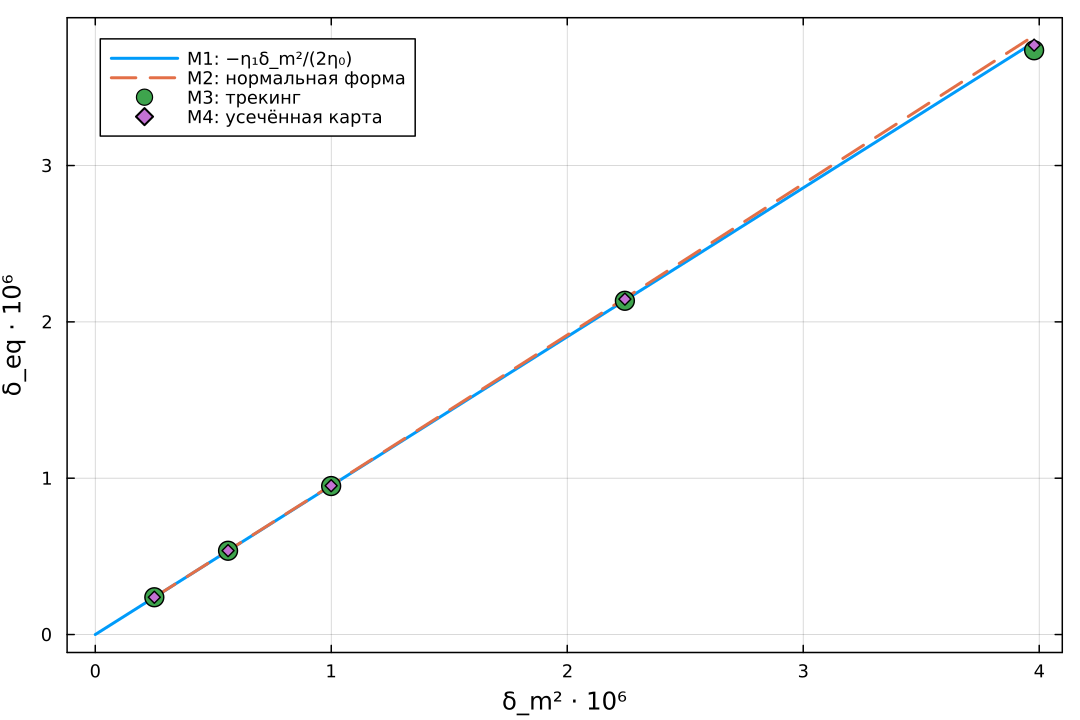
\includegraphics[width=0.8\textwidth]{figs/fig_A_delta_eq.png}
\caption{Тест A, модели \Mone--\Mfour. Равновесный сдвиг $\deq$ ($10^{-6}$) в зависимости от квадрата синхротронной амплитуды $\delta_m^2$ ($10^{-6}$), $J_x=J_y=0$. Линия --- формула \Mone{} с наклоном $-\eta_1/(2\eta_0)$; штрих --- нормальная форма \Mtwo{} при действиях начальной точки; круги --- трекинг \Mthree{}, ромбы --- усечённая карта \Mfour{}, по \vNA{} оборотов каждая. Зависимость линейна по $\delta_m^2$ и проходит через нуль: при тонком ВЧ постоянной добавки нет. Отклонение от прямой при $\delta_m\gtrsim1.5\cdot10^{-3}$ --- вклад следующего порядка по $\delta_m^2$.}
\end{figure}

\paragraph{Что следует.}
(1) При $\delta_m\le10^{-3}$ все модели совпадают в пределах $0.5\,\%$; \Mone{} и \Mthree{} --- в пределах $0.25\,\%$. (2) Свободного члена нет: при тонком ВЧ $\deq\to0$ при $\delta_m\to0$. (3) Отклонение \Mthree{} от \Mone{} растёт примерно как $\delta_m^2$ ($1.4\,\%$ при $\delta_m=2\cdot10^{-3}$, $\hat\varphi=0.41$): это члены $O(\delta_m^4)$ --- $\eta_2\delta^3$ в $\tau$, нелинейность ВЧ выше $\hat\varphi^2$ и т.\,п., не входящие ни в \Mone, ни в \Mtwo. Поправка $\hat\varphi^2/32$ (\Mone$_\varphi$) мала ($\le0.5\,\%$) и улучшает согласие. (4) \Mtwo{} отличается от \Mone{} не коэффициентами ($10^{-6}$), а аргументом: действие $J_s$ начальной точки соответствует $\delta_m^{(2)}=\sigma_\delta\sqrt{2J_s}$, которое на $\sim0.5\,\%$ больше амплитуды первой гармоники (табл.~\ref{tab:Amean}); при равных $\delta_m$ \Mone{} и \Mtwo{} совпадают.

\begin{table}[H]\centering\small
\caption{Тест A, детали оценки \Mthree. $\deq$ из гармонического фита и простое среднее по целому числу синхротронных периодов ($10^{-6}$); разность оценок по половинам ряда ($10^{-6}$); среднеквадратичный остаток фита (безразм.); амплитуда $\delta_m$ по \Mtwo{} ($\sigma_\delta\sqrt{2J_s}$) и из фита \Mthree{} ($10^{-3}$).}\label{tab:Amean}
\begin{tabular}{ccccccc}
\toprule
$\delta_{m0}$ & фит & среднее по периодам & пол.1 $-$ пол.2 & rms остатка & $\delta_m^{(2)}$ & $\delta_m^{(3)}$\\
\midrule
\tabin{gen/tabAmean.tex}
\bottomrule
\end{tabular}
\end{table}
Простое среднее отличается от фита на $\sim1$--$3\,\%$: оно чувствительно к остаточному незакрытому участку периода и ко второй гармонике (раздел~\ref{sec:time}).

\begin{table}[H]\centering\small
\caption{Синхротронный тюн. $J_s$ --- действие нормальной формы ($10^{-6}$\,м); $Q_s$ из \Mthree{} (фит), из нормальной формы \Mtwo{} ($Q_s-\partial h_4/\partial J_s/2\pi$) и по формуле $Q_s^{(0)}(1-\hat\varphi^2/16)$ с $\hat\varphi$ из \Mthree; разности с \Mthree.}\label{tab:Qs}
\begin{tabular}{cccccccc}
\toprule
$\delta_{m0}$ & $\hat\varphi$ & $J_s$ & $Q_s^{(3)}$ & $Q_s^{(2)}$ & $Q_s$ (ф-ла) & $\Delta Q^{(2)}$ & $\Delta Q^{\rm ф}$\\
\midrule
\tabin{gen/tabQs.tex}
\bottomrule
\end{tabular}
\end{table}
Нелинейный сдвиг синхротронного тюна ($\Delta Q_s/Q_s$ до $-1\,\%$) воспроизводится нормальной формой и формулой $1-\hat\varphi^2/16$ с точностью $\lesssim10^{-6}$ по $Q_s$.

%==========================================================================
\section{Тест B: вклад бетатронных колебаний}
$\delta_m=\vdmB$ (мал, чтобы вклад $\eta_1\delta_m^2$ не маскировал $\Lambda$), бетатронная амплитуда $A_x$ или $A_y$ от 5 до 20\,мм; $N=\vNB$ оборотов.
\begin{table}[H]\centering\footnotesize\setlength{\tabcolsep}{3pt}
\caption{Тест B. $A$ --- начальная амплитуда, мм; $J^{\rm CS}$ и $J^{\rm NF}$ --- действия ($10^{-6}$\,м); $\Lambda$ по \Mone, \Mtwo{} ($-\eta_0 d_kJ_k$) и из трекинга \Mthree{} ($10^{-6}$); $\deq$ по моделям ($10^{-6}$); $\Delta_i=M_i/M3-1$, \%.}\label{tab:B}
\begin{tabular}{cccccccccccc}
\toprule
пл. & $A$ & $J^{\rm CS}$ & $J^{\rm NF}$ & $\Lambda^{(1)}$ & $\Lambda^{(2)}$ & $\Lambda^{(3)}$ & \Mone & \Mtwo & \Mthree & $\Delta_1$ & $\Delta_2$\\
\midrule
\tabin{gen/tabB.tex}
\bottomrule
\end{tabular}
\end{table}

\begin{figure}[H]\centering
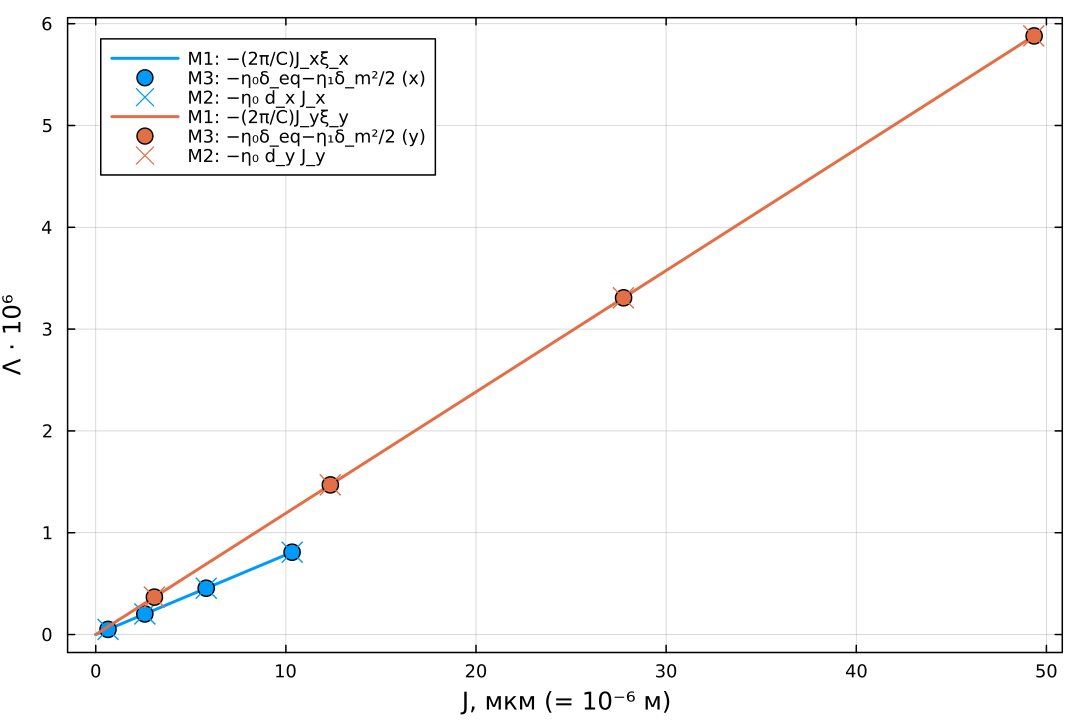
\includegraphics[width=0.8\textwidth]{figs/fig_B_lambda.png}
\caption{Тест B, модели \Mone--\Mthree. Относительное удлинение пути $\Lambda$ ($10^{-6}$) в зависимости от бетатронного действия $J$ ($10^{-6}$\,м) при $\delta_m=3\cdot10^{-4}$. Линии --- \Mone: $-(2\pi/C)J\xi$; круги --- \Mthree, $\Lambda=-\eta_0\deq-\eta_1\delta_m^2/2$ по \vNB{} оборотам; кресты --- \Mtwo. Линейность по $J$ и наклон $-2\pi\xi/C$ подтверждают связь удлинения пути с хроматичностью.}
\end{figure}

\paragraph{Что следует.} Для обеих плоскостей и всех амплитуд \Mone, \Mtwo{} и \Mthree{} совпадают в пределах $0.05\,\%$; $\Lambda$ из трекинга линейна по $J$ с наклоном $-2\pi\xi/C$ с той же точностью. Вертикальный вклад больше горизонтального из-за большей $|\xi_y|$ и, главное, большего действия при той же амплитуде ($\beta_y<\beta_x$ в точке наблюдения). Небольшое различие $J^{\rm CS}$ и $J^{\rm NF}$ ($\sim10^{-3}$ отн.) --- нелинейная поправка к действию и связь через дисперсию; оно объясняет основную часть различия \Mone{} и \Mtwo.

\begin{table}[H]\centering\small
\caption{Бетатронный тюн в тесте B: из БПФ трекинга \Mthree{} и из нормальной формы \Mtwo{} ($Q_k-\partial h_4/\partial J_k/2\pi$, дробная часть, приведённая к $[0,\frac12]$); $J^{\rm NF}$ в $10^{-6}$\,м.}
\begin{tabular}{cccccc}
\toprule
пл. & $A$, мм & $J^{\rm NF}$ & $Q^{(3)}$ & $Q^{(2)}$ & разность\\
\midrule
\tabin{gen/tabBQ.tex}
\bottomrule
\end{tabular}
\end{table}

%==========================================================================
\section{Установление среднего во времени}\label{sec:time}
$\deq$ --- среднее по бесконечному времени. В эксперименте и в трекинге доступно конечное число оборотов, поэтому важно, как быстро среднее устанавливается. Имеются два масштаба: бетатронный (период $\sim1$--$2$ оборота, $Q_{x,y}\approx0.46$) и синхротронный ($T_s\approx\vTs$ оборота).

\subsection{Быстрое бетатронное усреднение длины пути}
\begin{figure}[H]\centering
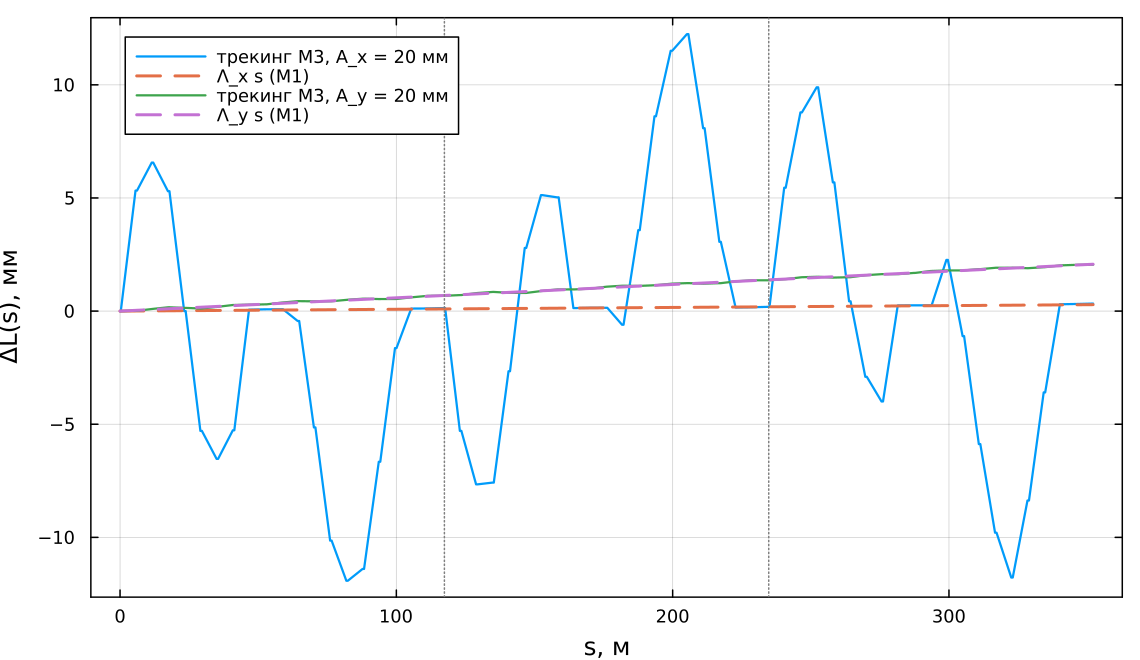
\includegraphics[width=0.85\textwidth]{figs/fig_fast_within_turn.png}
\caption{Модель \Mthree, ВЧ выключено, $\delta=0$. Накопленное удлинение пути $\Delta L(s)=-l(s)$ (мм) вдоль трёх оборотов (ось $s$, м; пунктир --- границы оборотов) для бетатронной амплитуды 20\,мм по $x$ ($J_x=\vJxFast\cdot10^{-6}$\,м) и по $y$ ($J_y=\vJyFast\cdot10^{-6}$\,м). Штрихи --- $\Lambda s$ с $\Lambda$ по \Mone. По $x$ доминирует член первого порядка $\int x_\beta/\rho\,\mathrm{d}s$ (размах $\sim\pm1$\,см), который знакопеременен по бетатронной фазе и почти полностью сокращается за оборот (в точке наблюдения $D_x\approx0$); остаётся квадратичный по амплитуде вековой член $\Lambda s$, на четыре порядка меньший. По $y$ члена первого порядка нет, и $\Delta L(s)$ сразу следует прямой $\Lambda_ys$ с малой модуляцией (наклоны в квадруполях).}
\end{figure}

\begin{figure}[H]\centering
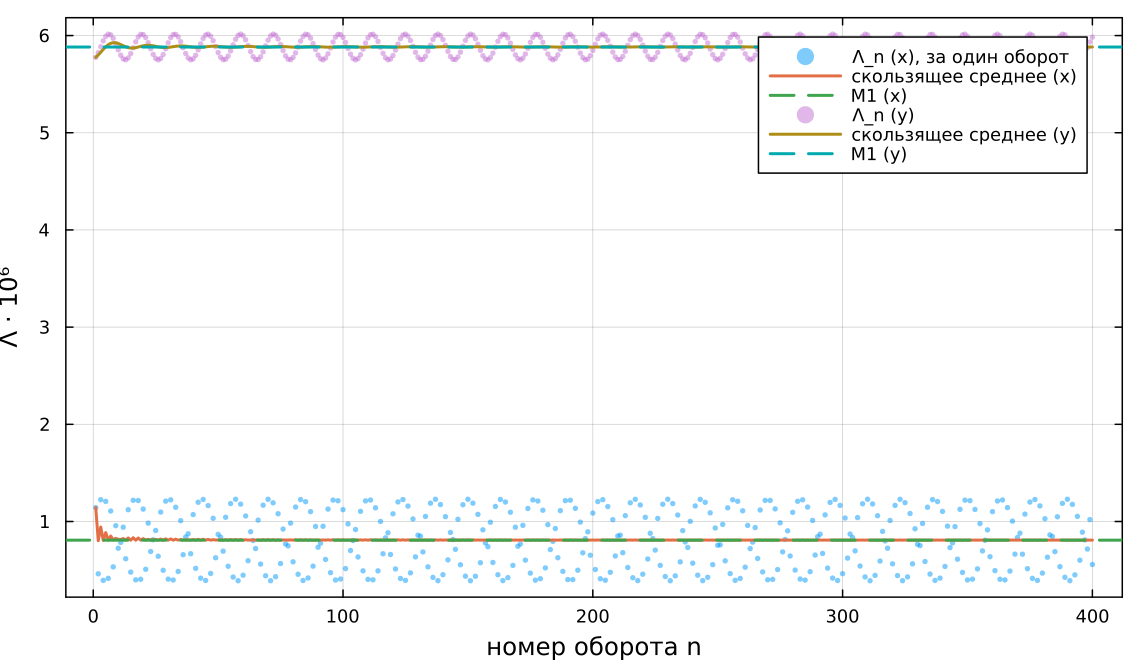
\includegraphics[width=0.85\textwidth]{figs/fig_fast_turns.png}
\caption{Модель \Mthree, ВЧ выключено, $\delta=0$, амплитуда 20\,мм. Точки --- удлинение пути $\Lambda_n=-\Delta l_n/C$ за отдельный $n$-й оборот ($10^{-6}$); линии --- скользящее среднее $\frac1N\sum_{n\le N}\Lambda_n$; штрих --- \Mone. За один оборот $\Lambda_n$ колеблется с бетатронной фазой (разброс $\vLamXspread\cdot10^{-6}$ по $x$, $\vLamYspread\cdot10^{-6}$ по $y$), среднее за \vNf{} оборотов: $x$: $\vLamXfastTr$ против $\vLamXfast$ (\Mone); $y$: $\vLamYfastTr$ против $\vLamYfast$ ($10^{-6}$). Бетатронное усреднение завершается за десятки оборотов --- много быстрее синхротронного, поэтому в продольном движении $\Lambda$ действует как постоянная.}
\end{figure}

\subsection{Медленное синхротронное усреднение}
\begin{figure}[H]\centering
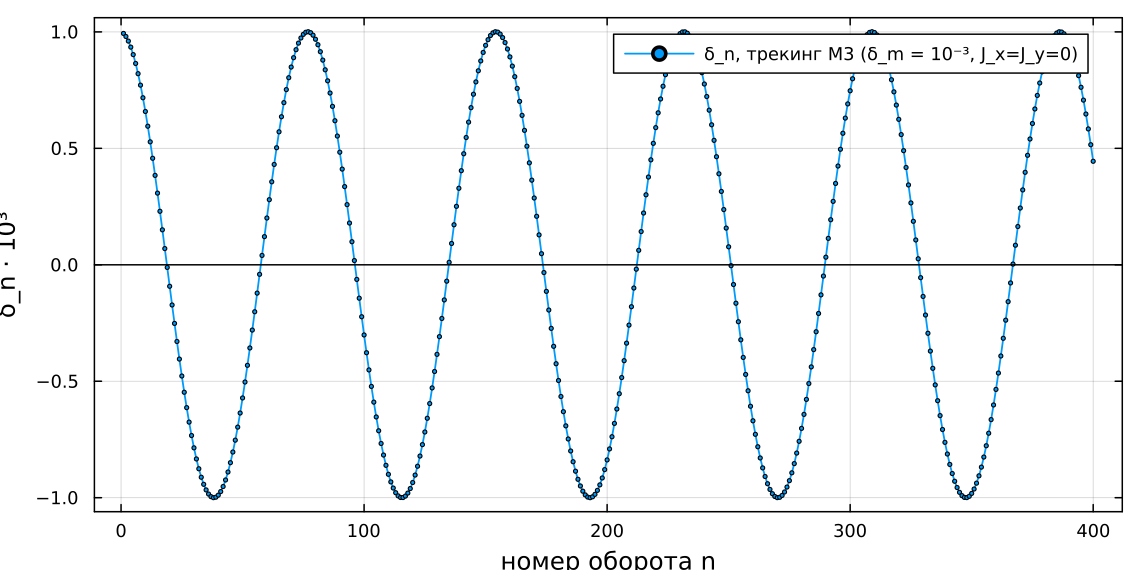
\includegraphics[width=0.85\textwidth]{figs/fig_T_series.png}
\caption{Модель \Mthree. Временной ряд $\delta_n$ ($10^{-3}$) в точке ВЧ-удара, $\delta_m=10^{-3}$, $J_x=J_y=0$, первые 400 оборотов. Колебание с периодом $T_s\approx\vTs$ оборота; сдвиг центра $\deq\approx10^{-6}$ на три порядка меньше амплитуды и на графике не виден --- он выделяется только усреднением.}
\end{figure}

\begin{figure}[H]\centering
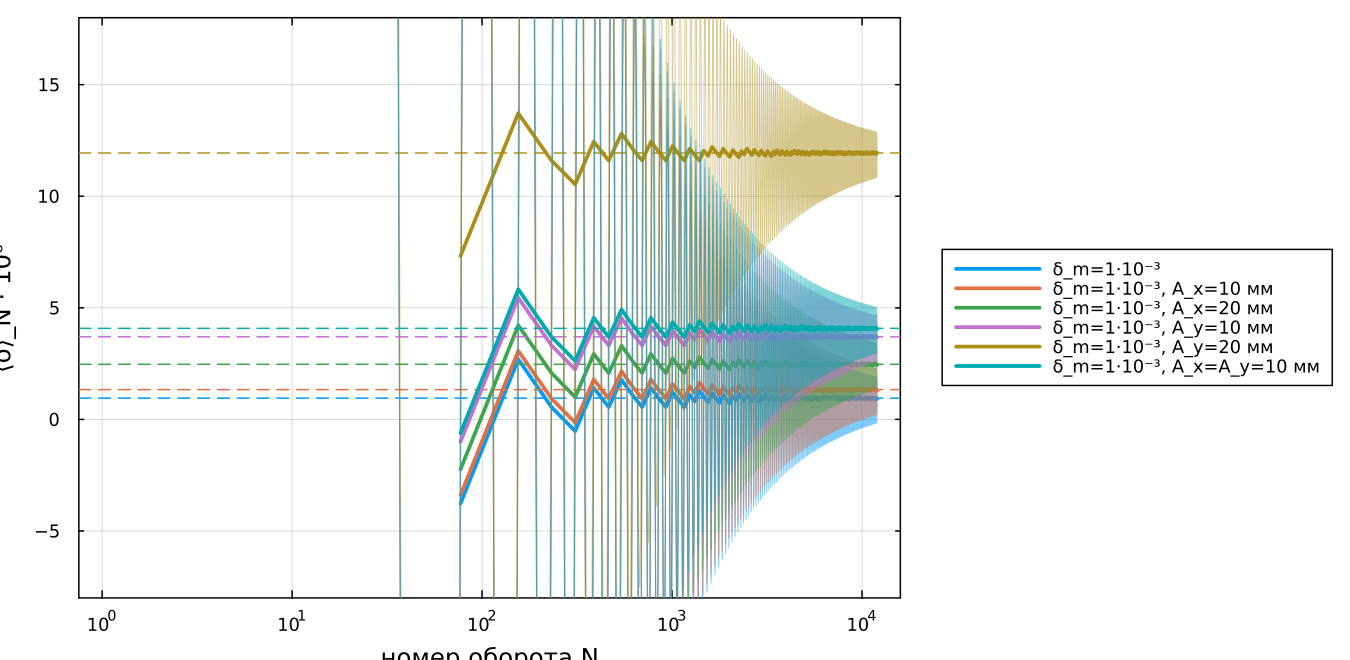
\includegraphics[width=0.85\textwidth]{figs/fig_T_runmean.png}
\caption{Модель \Mthree. Скользящее среднее $\langle\delta\rangle_N=\frac1N\sum_{n=1}^N\delta_n$ ($10^{-6}$) в зависимости от числа оборотов $N$ (лог. шкала) для $\delta_m=10^{-3}$ и разных бетатронных амплитуд; серые штрихи --- \Mtwo{} для каждого случая. Тонкие линии --- простое скользящее среднее; толстые --- среднее по целому числу синхротронных периодов $N=kT_s$ ($T_s$ --- измеренный период данного случая); штрихи --- \Mtwo{} того же цвета. Простое среднее осциллирует с периодом $T_s$ и огибающей $\delta_m/(N\sin\pi Q_s)$: при $N=\vNT$ его отклонение ещё $\vSimpleErrEnd$, т.\,е. сравнимо с самим $\deq$. Среднее по целым периодам сходится к уровню \Mtwo{} на порядок быстрее. Бетатронные амплитуды сдвигают уровень на $-\Lambda/\eta_0$ (до $11\cdot10^{-6}$ при $A_y=20$\,мм), не меняя характера сходимости: она определяется синхротронным колебанием.}
\end{figure}

\begin{table}[H]\centering\footnotesize\setlength{\tabcolsep}{3pt}
\caption{Сходимость скользящего среднего (\Mthree). Действия нормальной формы $J_x,J_y,J_s$ ($10^{-6}$\,м); $\deq$ по \Mone, \Mtwo, \Mthree{} (фит по всему ряду), $10^{-6}$; $|\langle\delta\rangle_N-\deq^{(2)}|$ при $N=10^2,10^3,10^4$. $N_{\max}=\vNT$.}\label{tab:conv}
\begin{tabular}{lccccccccc}
\toprule
случай & $J_x$ & $J_y$ & $J_s$ & \Mone & \Mtwo & \Mthree & $N=10^2$ & $10^3$ & $10^4$\\
\midrule
\tabin{gen/tabConv.tex}
\bottomrule
\end{tabular}
\end{table}

\begin{figure}[H]\centering
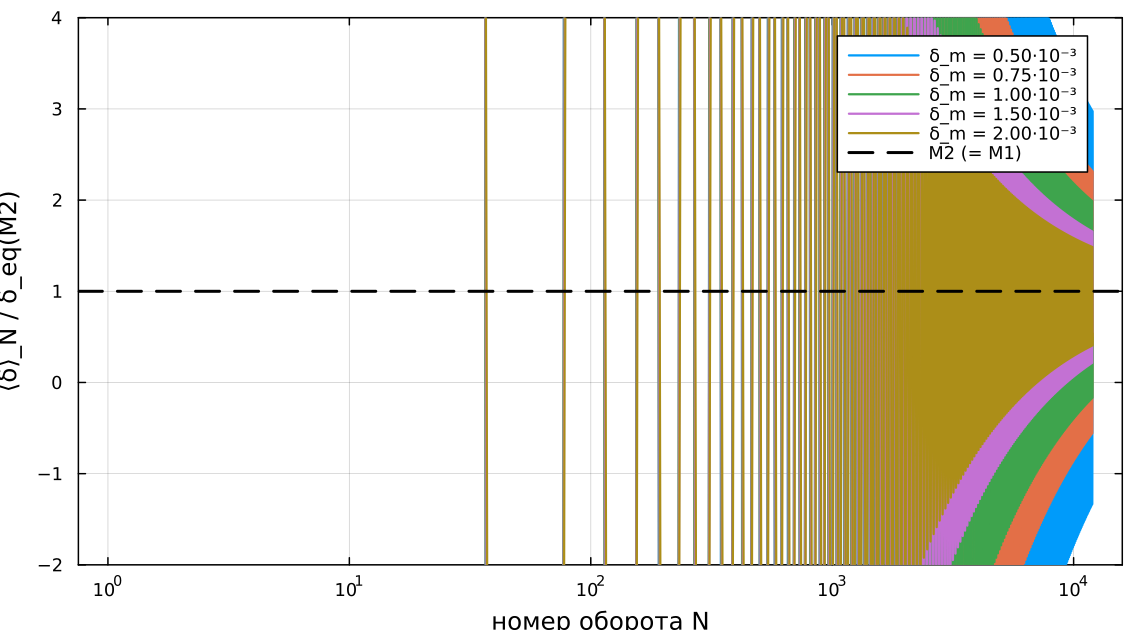
\includegraphics[width=0.85\textwidth]{figs/fig_T_runmean_dm.png}
\caption{Модель \Mthree, $J_x=J_y=0$. Скользящее среднее, нормированное на $\deq$ по \Mtwo{}, для пяти синхротронных амплитуд. Нормированные кривые почти совпадают: абсолютная ошибка среднего $\propto\delta_m$, а $\deq\propto\delta_m^2$, поэтому относительная ошибка $\propto1/(\delta_m N)$ --- при малых амплитудах сходимость по относительной точности медленнее.}
\end{figure}

\begin{figure}[H]\centering
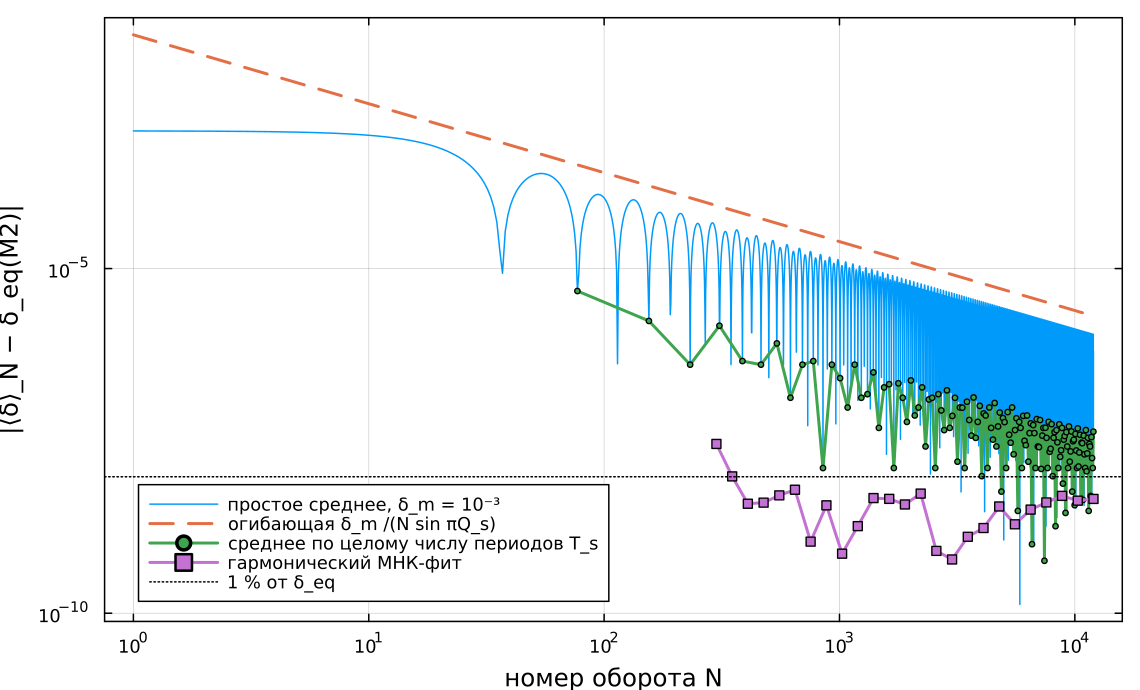
\includegraphics[width=0.85\textwidth]{figs/fig_T_convergence.png}
\caption{Модель \Mthree, $\delta_m=10^{-3}$, $J=0$. Ошибка $|\langle\delta\rangle_N-\deq^{(2)}|$ (безразм.) в зависимости от $N$ (лог.--лог.). Простое среднее (синяя линия) ограничено огибающей $\delta_m/(N\sin\pi Q_s)$ (штрих) --- закон $1/N$; для точности 1\,\% от $\deq$ (пунктир) ему нужно $N\approx\vNsimpleOnePct$ оборотов, за $\vNT$ оборотов ошибка $\vSimpleErrEnd$. Среднее по целому числу периодов (зелёные точки) исключает основную гармонику; остаётся вклад второй гармоники и неточности периода, ошибка при $N=\vNT$ --- $\vPmErrEnd$ (4\,\%). Гармонический МНК-фит (квадраты), явно содержащий первую и вторую гармоники и подгоняющий частоту, держится ниже 1\,\% начиная с $N=\vNfitOnePct$ (5 периодов), при $N=\vNT$ ошибка $\vFitErrEnd$. Поэтому в таблицах используется фит. Существенно, что частота берётся измеренной: усреднение по «целым» периодам с линейным $Q_s$ вместо амплитудно-зависимого ($\Delta Q_s/Q_s=-0.3\,\%$ при $\delta_m=10^{-3}$) за 155 периодов набирает рассогласование в 0.4 периода и даёт $\vMthreeMean\cdot10^{-6}$ вместо $0.95\cdot10^{-6}$.}
\end{figure}

\begin{figure}[H]\centering
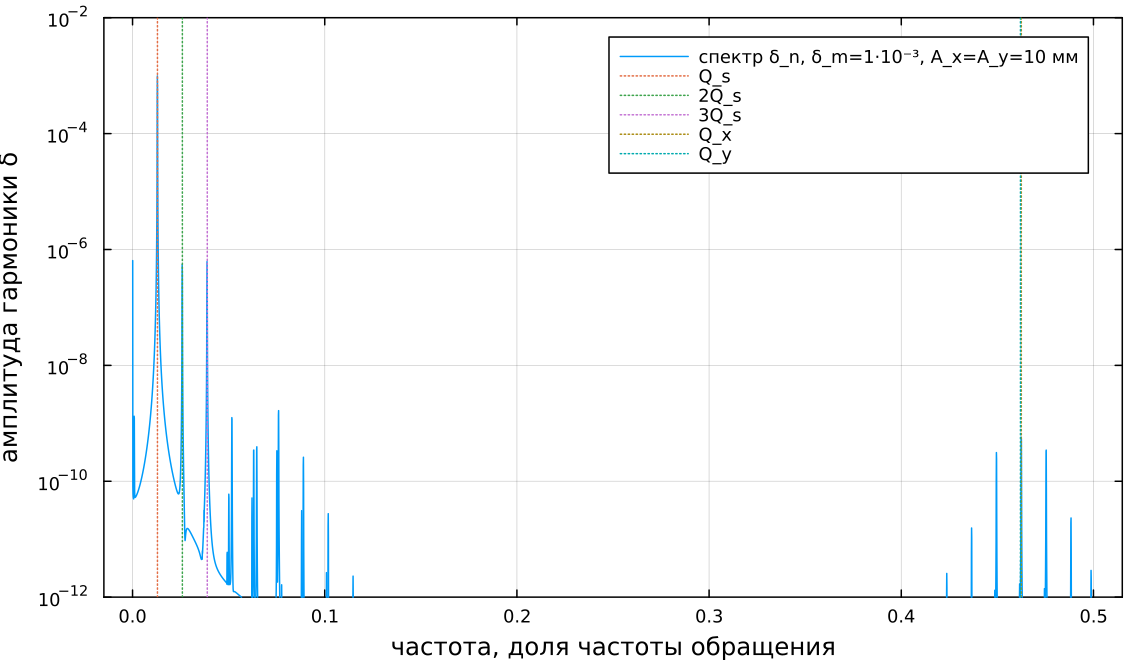
\includegraphics[width=0.85\textwidth]{figs/fig_T_spectrum.png}
\caption{Модель \Mthree, $\delta_m=10^{-3}$, $A_x=A_y=10$\,мм. Амплитудный спектр $\delta_n$ (окно Ханна, \vNT{} оборотов; ось частот --- в долях частоты обращения). Доминирует линия $Q_s$ с гармониками $2Q_s$, $3Q_s$ (нелинейность продольного движения); бетатронные линии на $Q_{x,y}$ на много порядков слабее: $\delta$ меняется только в ВЧ-ударе, а бетатронная модуляция времени прихода мала. Поэтому бетатронная часть усреднения на $\delta$ практически не сказывается, и $\Lambda$ входит в $\deq$ только через сдвиг центра синхротронного колебания.}
\end{figure}

\begin{figure}[H]\centering
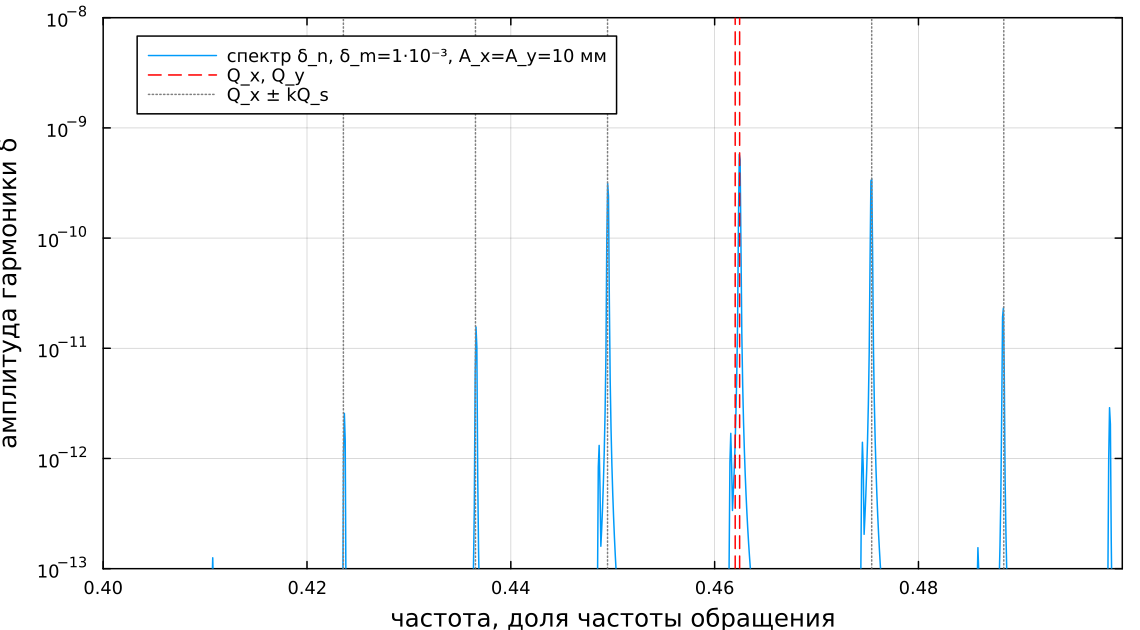
\includegraphics[width=0.85\textwidth]{figs/fig_T_spectrum_beta.png}
\caption{Модель \Mthree, $\delta_m=10^{-3}$, $A_x=A_y=10$\,мм. Участок спектра $\delta_n$ около бетатронных частот (те же данные, что на предыдущем рисунке). Линии лежат на $Q_{x,y}\pm kQ_s$ (пунктир): бетатронная модуляция $\delta$ возникает через дисперсию и время прихода в ВЧ-удар и модулирована синхротронной фазой. Наибольшая амплитуда $\vbetaLineMax$ --- на три--четыре порядка меньше $\deq$; быстрая составляющая усредняется за несколько оборотов и на $\deq$ не влияет.}
\end{figure}

\subsection{Сохранение фазового объёма: \Mthree{} против \Mfour}
\begin{figure}[H]\centering
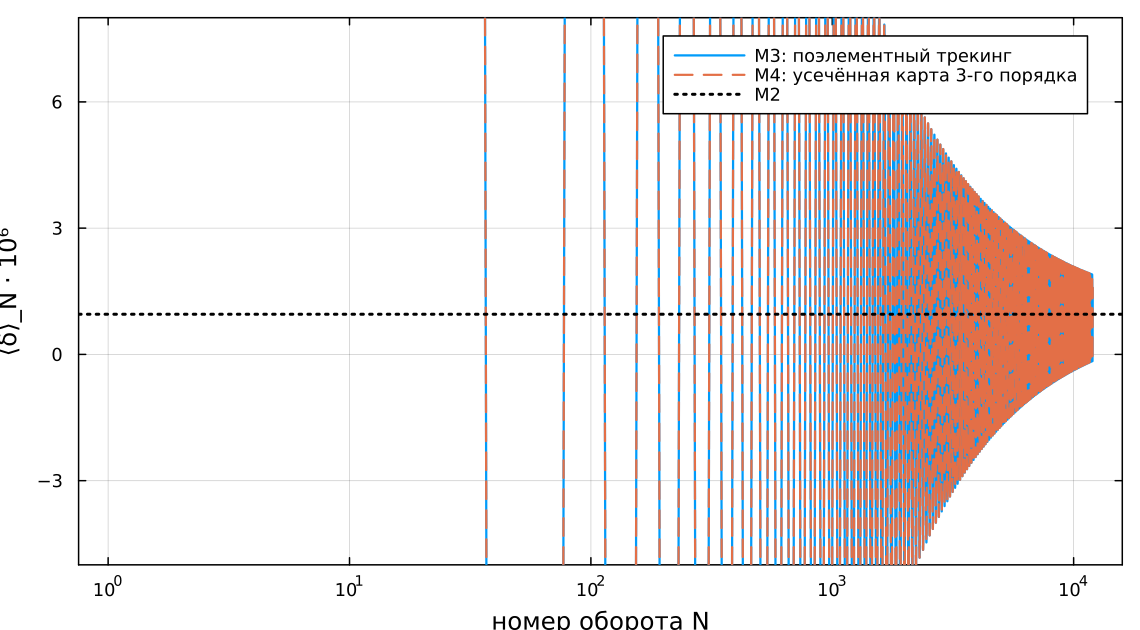
\includegraphics[width=0.85\textwidth]{figs/fig_M3_M4.png}
\caption{Модели \Mthree{} и \Mfour, $\delta_m=10^{-3}$, $J=0$. Простое скользящее среднее $\langle\delta\rangle_N$ ($10^{-6}$) за \vNA{} оборотов; пунктир --- \Mtwo. Кривые практически совпадают: несимплектичность усечённой карты за это время не успевает изменить амплитуду. Оценки фитом: \Mthree{} $\vMthreeFit$, \Mfour{} $\vMfourFit$ ($10^{-6}$), разность $0.2\,\%$ --- член четвёртого порядка, отсутствующий в усечённой карте. При больших $\delta_m$ разность растёт (табл.~\ref{tab:A}, $\Delta_4$).}
\end{figure}

%==========================================================================
\section{Выводы}
\begin{enumerate}
\item При тонком ВЧ формула $\deq=-(\eta_1\delta_m^2/2+\Lambda)/\eta_0$, $\Lambda=-(2\pi/C)(J_x\xi_x+J_y\xi_y)$ подтверждается средним $\delta$ по тору нормальной формы произведения Ли: коэффициенты $\partial\deq/\partial J_{x,y,s}$ совпадают с формулой с относительной точностью $10^{-6}$.
\item Трекинг (\Mthree) подтверждает формулу в пределах $0.25\,\%$ при $\delta_m\le10^{-3}$; при больших амплитудах различие растёт как $\delta_m^2$ (поправки следующего порядка), множитель $1-\hat\varphi^2/32$ уменьшает его.
\item Бетатронный вклад линеен по действию и определяется полной хроматичностью; бетатронное усреднение длины пути происходит за десятки оборотов, синхротронное медленно: ошибка простого среднего $\approx\delta_m/(N\sin\pi Q_s)$, для 1\,\% при $\delta_m=10^{-3}$ нужно $\sim\vNsimpleOnePct$ оборотов; гармонический фит с измеренной частотой даёт 1\,\% за $\sim\vNfitOnePct$ оборотов.
\item Нелинейный синхротронный тюн из нормальной формы совпадает с трекингом и с $1-\hat\varphi^2/16$ с точностью $<10^{-6}$; бетатронные тюны из нормальной формы и трекинга совпадают до $3\cdot10^{-6}$.
\item Постоянной добавки $\sim10^{-7}$, наблюдавшейся ранее, при тонком ВЧ нет; влияние конечного резонатора --- отдельная задача.
\end{enumerate}

\appendix
\section{Методическое приложение}
\begin{itemize}
\item \Mone: аналитические выражения \eqref{eq:M1}; $\eta_0,\eta_1$ --- из разложения времени пролёта по $\delta$ на замкнутой дисперсионной орбите отображения магнитной структуры; $\xi$ --- производная тюна по $\delta$ (центральная разность по замкнутой орбите).
\item \Mtwo: произведение факторов Драгта--Финна магнитных элементов и тонкого ВЧ; нормальная форма на генераторах по разд.~\ref{sec:nf}; действия в метрах.
\item \Mthree: неразложенный гамильтониан $H=-(1+hx)\sqrt{(1+\delta)^2-p_x^2-p_y^2}+\dots$ с энергетическим членом, симплектическая неявная схема средней точки, шаг $\le0.1$\,м; ВЧ --- точный тонкий удар.
\item \Mfour: полиномиальное разложение того же произведения до степени 3, итерации без симплектизации.
\item Оценка $\deq$, $\delta_m$, $Q_s$, погрешностей --- разд.~\ref{sec:method}.
\end{itemize}

\end{document}
